\documentclass[9pt]{extarticle}

% ---- packages (all standard, pdflatex-friendly) ----
\usepackage[a4paper,top=1.1cm,bottom=1.0cm,left=1.3cm,right=1.3cm]{geometry}
\usepackage{graphicx}
\usepackage{xcolor}
\usepackage{enumitem}
\usepackage{multicol}
\usepackage[most]{tcolorbox}
\usepackage{helvet}
\renewcommand{\familydefault}{\sfdefault}

% ---- colours ----
\definecolor{ink}{HTML}{0F1B2D}
\definecolor{accent}{HTML}{0B6BCB}
\definecolor{warm}{HTML}{E07A1F}
\definecolor{softgrey}{HTML}{EDF1F6}
\color{ink}

\pagestyle{empty}
\setlength{\parindent}{0pt}
\setlength{\parskip}{3pt}
\setlength{\columnsep}{0.7cm}

% compact section header (text, small gap, then a clean rule below it)
\newcommand{\head}[1]{\vspace{3pt}{\color{accent}\bfseries #1}\par\vspace{2pt}{\color{accent}\hrule height 0.6pt}\vspace{4pt}}

% tighter itemize/enumerate
\setlist[itemize]{leftmargin=1.1em,itemsep=1.5pt,topsep=1.5pt,parsep=0pt}
\setlist[enumerate]{leftmargin=1.3em,itemsep=1.5pt,topsep=1.5pt,parsep=0pt}

\begin{document}

% =======================  TITLE  =======================
\begin{center}
    {\LARGE\bfseries How Predictable Is a Flow Traders Earnings Letter?}\\[3pt]
    {\color{warm}\normalsize Measuring the information content of eight quarters of CEO commentary}\\[1pt]
    {\footnotesize 8 quarterly letters (2023\,Q4\,--\,2025\,Q4) $\cdot$ n-gram + frequency + novelty $\cdot$ no neural nets --- every result is explainable}
\end{center}
\vspace{1pt}

% =======================  PREMISE BOX  =======================
\begin{tcolorbox}[colback=softgrey,colframe=accent,boxrule=1pt,arc=2pt,left=7pt,right=7pt,top=3pt,bottom=3pt]
\textbf{The question.} A market maker's edge is turning information into a position quickly. So a fair thing to ask of any recurring corporate text is: \emph{how much of it is actually new?} If a letter is mostly boilerplate, a reader can skip to the few sentences that carry signal --- and a simple model should be able to anticipate the rest. This is a small experiment to quantify exactly that on Flow's own filings.
\end{tcolorbox}
\vspace{2pt}

% =======================  TWO COLUMNS  =======================
\begin{multicols}{2}

\head{What we did}
Extracted the CEO commentary from eight consecutive quarterly releases, stripped tables and boilerplate, and treated each letter as a document. The goal was not a clever model --- it was to \emph{measure structure} with the plainest tools that still answer the question.

\head{How we did it}
\begin{enumerate}
    \item \textbf{Frequency + document-frequency:} rank content words by how often they occur \emph{and} in how many of the eight letters.
    \item \textbf{Trigram model:} learn which word follows which, so it can generate a plausible next-quarter opener.
    \item \textbf{Novelty / recycling:} per letter, the share of vocabulary seen in a prior letter (theme reuse) vs.\ repeated \emph{exact} phrasing (n-gram overlap).
    \item \textbf{Out-of-sample backtest:} train on the first seven letters, hide the eighth, and test how much of it the model calls.
\end{enumerate}

\columnbreak

\head{What we found}
\begin{itemize}
    \item \textbf{8} letters, \textbf{402} words each on average.
    \item \textbf{Six} content words appear in \emph{all eight} letters; more in seven of eight. The thematic vocabulary is stable.
    \item \textbf{48\%} of a letter's vocabulary is recycled from earlier letters --- and the share \emph{rises} over time.
    \item Yet only \textbf{7.8\%} of exact phrasing repeats: same themes, freshly rewritten sentences.
    \item \textbf{Backtest:} \textbf{80\%} of the model's top-15 predicted words appeared in the unseen eighth letter.
\end{itemize}

\head{Reading the result}
The signal-to-boilerplate ratio is low. Most of what a Flow letter ``says'' is predictable a quarter ahead; the genuinely new content sits in a handful of sentences. For a reader optimising for speed, that is the useful part --- most of the document compresses away.

\end{multicols}
\vspace{1pt}

% =======================  FIGURES  =======================
\begin{center}
\begin{minipage}{0.49\textwidth}\centering
    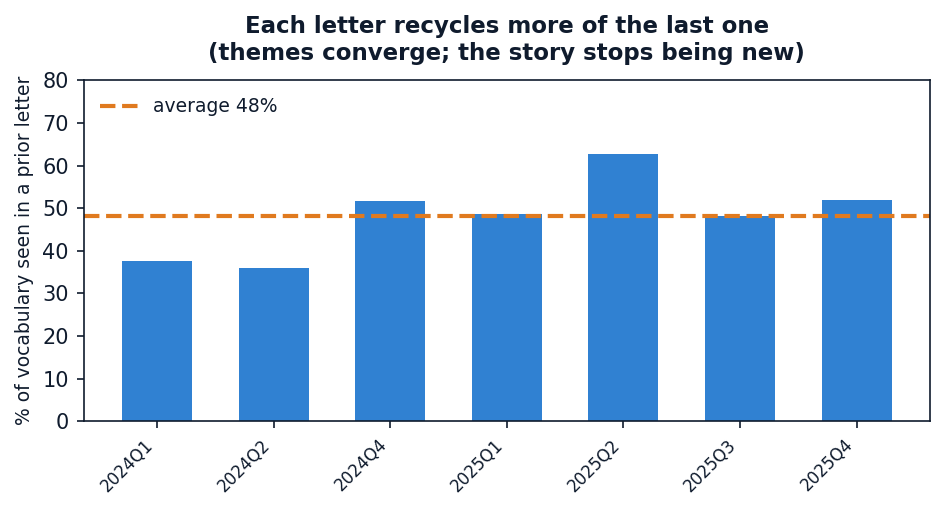
\includegraphics[width=\linewidth,height=4.6cm,keepaspectratio]{chart_recycling.png}
\end{minipage}\hfill
\begin{minipage}{0.49\textwidth}\centering
    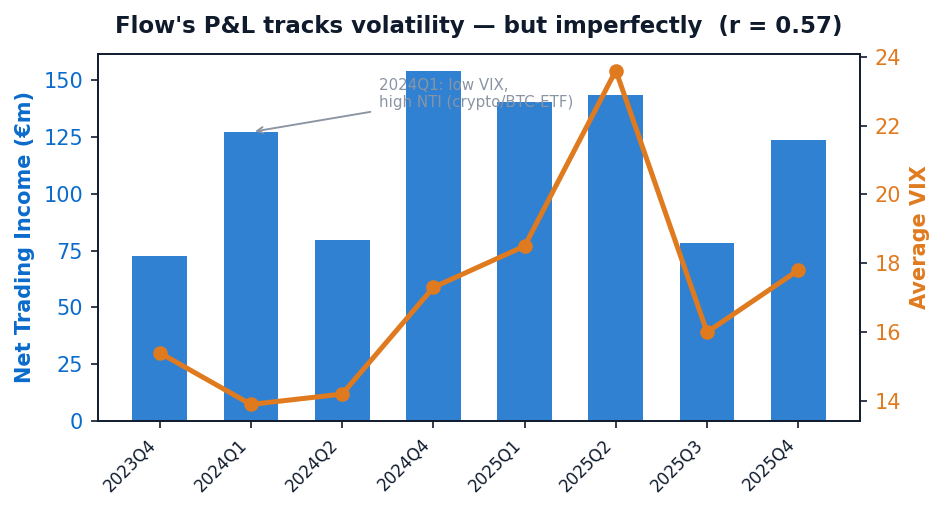
\includegraphics[width=\linewidth,height=4.6cm,keepaspectratio]{chart_nti_vix.png}
\end{minipage}
\end{center}
\vspace{2pt}

% =======================  PUNCHLINE  =======================
\begin{tcolorbox}[colback=ink,colframe=ink,arc=2pt,left=7pt,right=7pt,top=3pt,bottom=3pt]
\color{white}
\textbf{The point.} The \emph{language} is roughly 80\% predictable. The variable that actually drives the P\&L --- \textbf{volatility} --- is not: Net Trading Income tracks the VIX at only $r=0.57$, and 2024\,Q1 breaks the pattern outright (lowest VIX in the sample, near-highest income, carried by a countercyclical business line rather than by market swings). So the letter's real information content compresses to about one question --- \emph{was it volatile, and did the diversification offset hold?} Predictable prose, unpredictable returns: a clean illustration of where the exploitable information actually lives.
\end{tcolorbox}
\vspace{3pt}

% =======================  THE GAME (no hints)  =======================
\begin{center}
{\bfseries The wager: which \emph{five} words do you think recur most across all eight letters?}\\[5pt]
\underline{\hspace{2.9cm}}\quad\underline{\hspace{2.9cm}}\quad\underline{\hspace{2.9cm}}\quad\underline{\hspace{2.9cm}}\quad\underline{\hspace{2.9cm}}\\[3pt]
{\footnotesize\itshape Write your five. The model's ranked answer is sealed --- we compare over lunch.}
\end{center}

\end{document}
